\subsection{Zeitabhängigkeit der Lumineszenz} 
\authors{Gala Gottschalg, Sophia Ivaschuk}

Im zuvor beschriebenen Versuch wurden alle zwei Sekunden Intervall-Aufnahmen aufgenommen. Dabei wurden die vier Photographien untereinander verglichen und die Intensität der Lumineszenz ermittelt. Die Ergebnisse sind in Tabelle \ref{dsatable:Zeitabhaengigkeit} angegeben.

\begin{dsatable}
 \caption{Zeitabhängigkeit der Lumineszenz.}
 \centering
 \begin{tabular}{lr} % zwei Spalten
  \toprule
  Zeit &  Intensitätswert\\
  \midrule
  2 Sekunden      & 84.8746\\
  4 Sekunden      & 52.4111\\
  6 Sekunden      & 35.0930\\
  8 Sekunden      & 24.4441\\
  \bottomrule
 \end{tabular}
 \label{dsatable:Zeitabhaengigkeit}
\end{dsatable}


Die rechte Spalte der Tabelle zeigt die relative Intensität der Lumineszenz im Versuchsverlauf. Wie man den Tabellenwerten entnehmen kann, ist der Verlauf der Intensitätskurve nicht linear. Stattdessen verringert sich die Intensität zunächst stärker, wobei anschließend die Abnahme von Bild zu Bild geringer wird, bis sie sich final einem Wert von null annähert und der Vorgang der Lumineszenz abgeschlossen ist.
Dies wird besonders in Abbildung \ref{fig:Intensitaet} deutlich, in der die Werte der Intensität dargestellt sind.

\begin{dsafigure}
 \centering
 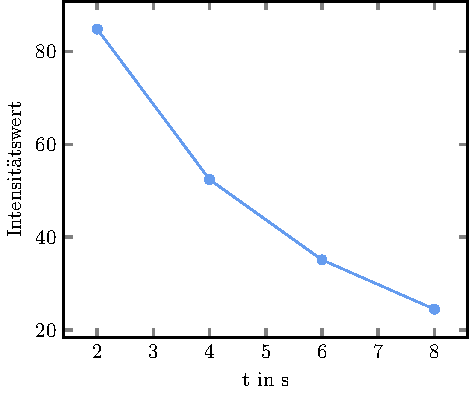
\includegraphics[width=\columnwidth]{Graph_Intensitaet.pdf}
 \caption{Verlauf der Intensitätswerte.}
 \label{fig:Intensitaet}
\end{dsafigure}


